\chapter{Theory}\label{chap:cms}


One of the most compelling questions in participle physics today is the hierarchy problem. The Randall Sundrum Kaluza Klein model proposes a solution in which the Planck scale is located on one membrane and the TeV scale a distance L away in a fourth spatial dimension. 

\begin{figure}[h]
	\centering
	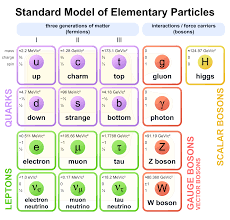
\includegraphics[width=0.5\textwidth]{figures/sm_blocks.png}
	\caption{The fundamental particles in the standard model of particle physics.}
	\label{fig:sm}
\end{figure}
\clearpage

\section{History of particle physics}

\newpage

\section{Standard Model Particle Interactions}

\newpage




Particles interact by exchanging force particles, all of which are spin-1 bosons in the Standard Model. The force particles are excitations of their corresponding fields. For the electromagnetic field, the force particle is the photon. The cross section of an interaction between particles is proportional to the scattering amplitude. In the simplest case of an electromagnetic interaction, an electron and muon collide with each other and exchange a photon. The coupling strength of the electromagnetic interaction is $e$, and the scattering amplitude is $sin^{-4}(\frac{\theta}/{2})$. This relationship to the scattering angle occurs because the mediation force particle is massless. In the weak force interactions, the mediating particle is not massless, since the mass of the $Z$ boson is 91 GeV and the mass of the $W$ boson is 80 GeV. Therefore, weak interactions are suppressed when $q^2 << {M^{2}}_{W}$.

\begin{figure}
	\centering
	\feynmandiagram [vertical=a to b] {
	  i1 [particle=\(e^{-}\)] -- [fermion] a -- [fermion] i2 [particle=\(e^{-}\)],
	  a -- [photon, edge label'=\(\gamma\)] b,
 	 f1 [particle=\(\mu^{-}\)] -- [anti fermion] b -- [anti fermion] f2 [particle=\(\mu^{-}\)],
	};
	\caption{An electron muon scattering interaction with scattering amplitude $e^2/q^2$ for a 1 photon exchange interaction.}
\end{figure}

\subsection{Electroweak Symmetry breaking}

The electroweak interaction is a unified description of the electromagnetic and weak forces. At high temperatures corresponding to an energy of 246 GeV, the electromagnetic and weak forces can be described by one force. Experiments finding the W and Z bosons confirmed some of the predictions of the theory. The electroweak force has four bosons before symmetry breaking occurs ($W_1$, $W_2$, $W_3$ and $B$). After electroweak symmetry breaking, the $W$ boson is a combination of the first 2 electroweak bosons (Equation~\ref{eq:w}) and the photon and $W$ and $Z$ bosons are a combination of the latter 2 (Equation~\ref{eq:zgamma} 

\begin{equation}
	W^{\pm} = \frac{1}{\sqrt{2}}
	\begin{pmatrix}
		W_1 \mp iW_2
	\end{pmatrix}
	\label{eq:w}
\end{equation}


\begin{equation}
	\begin{pmatrix}
		\gamma \\
		Z 
	\end{pmatrix} = \begin{pmatrix}
		\cos{\theta_W} & \sin{\theta_W} \\
		-\sin{\theta_W} & \cos{\theta_W}
	\end{pmatrix}
	\begin{pmatrix}
		B \\
		W_3 
	\end{pmatrix}
	\label{eq:zgamma}
\end{equation}

where $\theta_W$ is the weak mixing angle, or "Weinberg angle", which is the angle relating $g'$ to $g$, as shown in Figure~\ref{fig:weinberg}.


\section{Beyond Standard Model}


\subsection{Searches for new physics}

The top quark is a key to our understanding of the missing puzzle piecs in the standard model. The top quark is the heaviest of the fundamental particles, and its 173 GeV mass is on the order of electroweak symmetry breaking. Therefore studying the top quark in high statistics experiments such as the LHC can reveal inconsistencies in the mass of $m_t$ from predictions, or can find exotic decay modes of the top, or can find exotic intermediate states that decay to the top quark.



Table \ref{fig:smtable} shows the SM particle interactions for the corresponding SM particles.

Figure \ref{fig:sm} shows the particles that are fundamental in the standard model of particles physics.

\begin{figure}[htbp!]
	\centering
	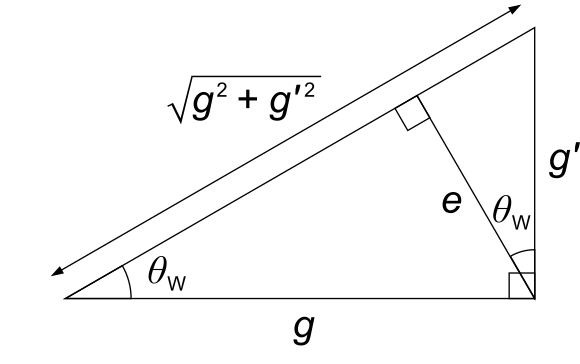
\includegraphics[width=0.5\textwidth]{figures/Weinberg_angle.png}
	\caption{The weak mixing angle $\theta_W$ is the angle relating $g'$ to $g$.}
	\label{fig:weinberg}
\end{figure}

 \begin{figure}[h!]
\centering
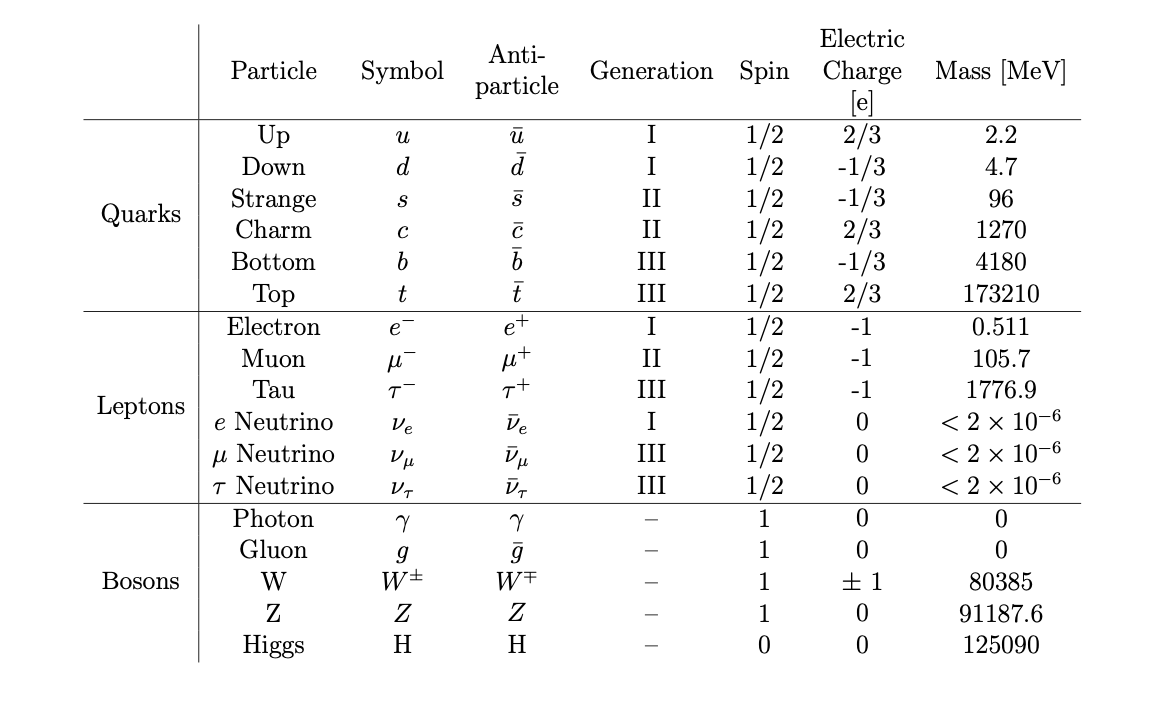
\includegraphics[width=0.8\textwidth]{figures/sm_table.png}
\caption{Table of SM particle interactions \textbf{to be replaced}.}
\label{fig:smtable}
\end{figure}





\subsection{Extra Dimensions}

One of the theories introduced to explain the hierarchy problem is the Kaluza-Klein gluon with an extra spacial dimension from the Randall-Sundrum (RS) framework. In the RS framework, there are two planes - the UV plane and the IR plane. The Planck scale is located on the UV plane, and the TeV scale is located on the IR plane. The two planes interact in the fifth spacial dimension, called the “bulk”. The Kaluza-Klein gluon has a signal comparable to SM QCD background with a luminosity of 100 fb$^{-1}$, which is comparable to the 137 fb$^{-1}$ luminosity of Run 2.

A diagram of the scale of the standard model forces to the planck scale is shown in Figure~\ref{fig:planck}. A diagram of the extra dimensions that are theorized to explain the large gap between the standard model forces and the Planck scale is shown in Figure~\ref{fig:rsbrane}.

\begin{figure}[h]
	\centering
	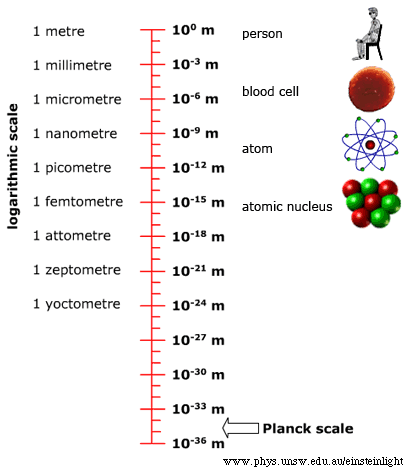
\includegraphics[width=0.5\textwidth]{figures/Planck_scale.png}
	\caption{Logarithmic scale of standard model forces and Planck scale~\cite{Planck_scale}.}
	\label{fig:planck}
\end{figure}

\begin{figure}[h]
	\centering
	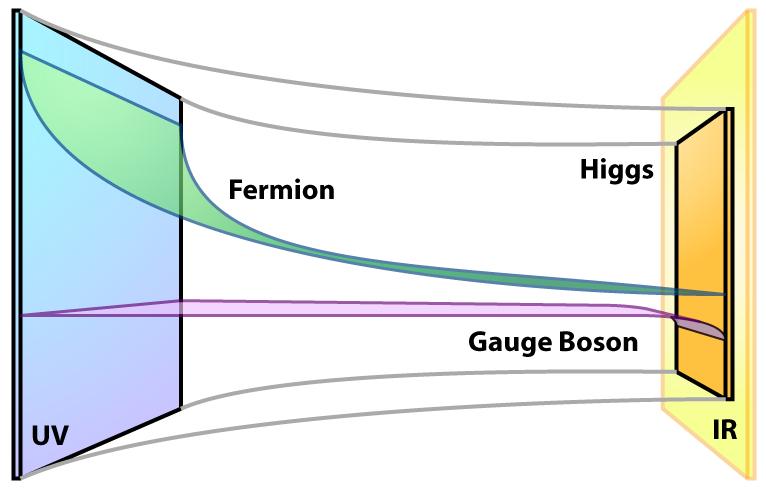
\includegraphics[width=0.75\textwidth]{figures/RSBrane.png}
	\caption{The extra spatial dimensions proposed in the Randall-Sundrum model~\cite{RSBrane}.}
	\label{fig:rsrbane}
\end{figure}

